\documentclass[twoside]{book}

% Packages required by doxygen
\usepackage{fixltx2e}
\usepackage{calc}
\usepackage{doxygen}
\usepackage[export]{adjustbox} % also loads graphicx
\usepackage{graphicx}
\usepackage[utf8]{inputenc}
\usepackage{makeidx}
\usepackage{multicol}
\usepackage{multirow}
\PassOptionsToPackage{warn}{textcomp}
\usepackage{textcomp}
\usepackage[nointegrals]{wasysym}
\usepackage[table]{xcolor}

% Font selection
\usepackage[T1]{fontenc}
\usepackage[scaled=.90]{helvet}
\usepackage{courier}
\usepackage{amssymb}
\usepackage{sectsty}
\renewcommand{\familydefault}{\sfdefault}
\allsectionsfont{%
  \fontseries{bc}\selectfont%
  \color{darkgray}%
}
\renewcommand{\DoxyLabelFont}{%
  \fontseries{bc}\selectfont%
  \color{darkgray}%
}
\newcommand{\+}{\discretionary{\mbox{\scriptsize$\hookleftarrow$}}{}{}}

% Page & text layout
\usepackage{geometry}
\geometry{%
  a4paper,%
  top=2.5cm,%
  bottom=2.5cm,%
  left=2.5cm,%
  right=2.5cm%
}
\tolerance=750
\hfuzz=15pt
\hbadness=750
\setlength{\emergencystretch}{15pt}
\setlength{\parindent}{0cm}
\setlength{\parskip}{3ex plus 2ex minus 2ex}
\makeatletter
\renewcommand{\paragraph}{%
  \@startsection{paragraph}{4}{0ex}{-1.0ex}{1.0ex}{%
    \normalfont\normalsize\bfseries\SS@parafont%
  }%
}
\renewcommand{\subparagraph}{%
  \@startsection{subparagraph}{5}{0ex}{-1.0ex}{1.0ex}{%
    \normalfont\normalsize\bfseries\SS@subparafont%
  }%
}
\makeatother

% Headers & footers
\usepackage{fancyhdr}
\pagestyle{fancyplain}
\fancyhead[LE]{\fancyplain{}{\bfseries\thepage}}
\fancyhead[CE]{\fancyplain{}{}}
\fancyhead[RE]{\fancyplain{}{\bfseries\leftmark}}
\fancyhead[LO]{\fancyplain{}{\bfseries\rightmark}}
\fancyhead[CO]{\fancyplain{}{}}
\fancyhead[RO]{\fancyplain{}{\bfseries\thepage}}
\fancyfoot[LE]{\fancyplain{}{}}
\fancyfoot[CE]{\fancyplain{}{}}
\fancyfoot[RE]{\fancyplain{}{\bfseries\scriptsize Generated by Doxygen }}
\fancyfoot[LO]{\fancyplain{}{\bfseries\scriptsize Generated by Doxygen }}
\fancyfoot[CO]{\fancyplain{}{}}
\fancyfoot[RO]{\fancyplain{}{}}
\renewcommand{\footrulewidth}{0.4pt}
\renewcommand{\chaptermark}[1]{%
  \markboth{#1}{}%
}
\renewcommand{\sectionmark}[1]{%
  \markright{\thesection\ #1}%
}

% Indices & bibliography
\usepackage{natbib}
\usepackage[titles]{tocloft}
\setcounter{tocdepth}{3}
\setcounter{secnumdepth}{5}
\makeindex

% Hyperlinks (required, but should be loaded last)
\usepackage{ifpdf}
\ifpdf
  \usepackage[pdftex,pagebackref=true]{hyperref}
\else
  \usepackage[ps2pdf,pagebackref=true]{hyperref}
\fi
\hypersetup{%
  colorlinks=true,%
  linkcolor=blue,%
  citecolor=blue,%
  unicode%
}

% Custom commands
\newcommand{\clearemptydoublepage}{%
  \newpage{\pagestyle{empty}\cleardoublepage}%
}

\usepackage{caption}
\captionsetup{labelsep=space,justification=centering,font={bf},singlelinecheck=off,skip=4pt,position=top}

%===== C O N T E N T S =====

\begin{document}

% Titlepage & ToC
\hypersetup{pageanchor=false,
             bookmarksnumbered=true,
             pdfencoding=unicode
            }
\pagenumbering{alph}
\begin{titlepage}
\vspace*{7cm}
\begin{center}%
{\Large My Project }\\
\vspace*{1cm}
{\large Generated by Doxygen 1.8.12}\\
\end{center}
\end{titlepage}
\clearemptydoublepage
\pagenumbering{roman}
\tableofcontents
\clearemptydoublepage
\pagenumbering{arabic}
\hypersetup{pageanchor=true}

%--- Begin generated contents ---
\chapter{Hierarchical Index}
\section{Class Hierarchy}
This inheritance list is sorted roughly, but not completely, alphabetically\+:\begin{DoxyCompactList}
\item \contentsline{section}{Person}{\pageref{class_person}}{}
\begin{DoxyCompactList}
\item \contentsline{section}{Contestant}{\pageref{class_contestant}}{}
\item \contentsline{section}{Mentor}{\pageref{class_mentor}}{}
\end{DoxyCompactList}
\item \contentsline{section}{Season}{\pageref{class_season}}{}
\item \contentsline{section}{Song}{\pageref{class_song}}{}
\item \contentsline{section}{The\+Voice}{\pageref{class_the_voice}}{}
\end{DoxyCompactList}

\chapter{Class Index}
\section{Class List}
Here are the classes, structs, unions and interfaces with brief descriptions\+:\begin{DoxyCompactList}
\item\contentsline{section}{\hyperlink{class_contestant}{Contestant} }{\pageref{class_contestant}}{}
\item\contentsline{section}{\hyperlink{class_mentor}{Mentor} }{\pageref{class_mentor}}{}
\item\contentsline{section}{\hyperlink{class_person}{Person} }{\pageref{class_person}}{}
\item\contentsline{section}{\hyperlink{class_season}{Season} }{\pageref{class_season}}{}
\item\contentsline{section}{\hyperlink{class_song}{Song} }{\pageref{class_song}}{}
\item\contentsline{section}{\hyperlink{class_the_voice}{The\+Voice} }{\pageref{class_the_voice}}{}
\end{DoxyCompactList}

\chapter{Class Documentation}
\hypertarget{class_contestant}{}\section{Contestant Class Reference}
\label{class_contestant}\index{Contestant@{Contestant}}
Inheritance diagram for Contestant\+:\begin{figure}[H]
\begin{center}
\leavevmode
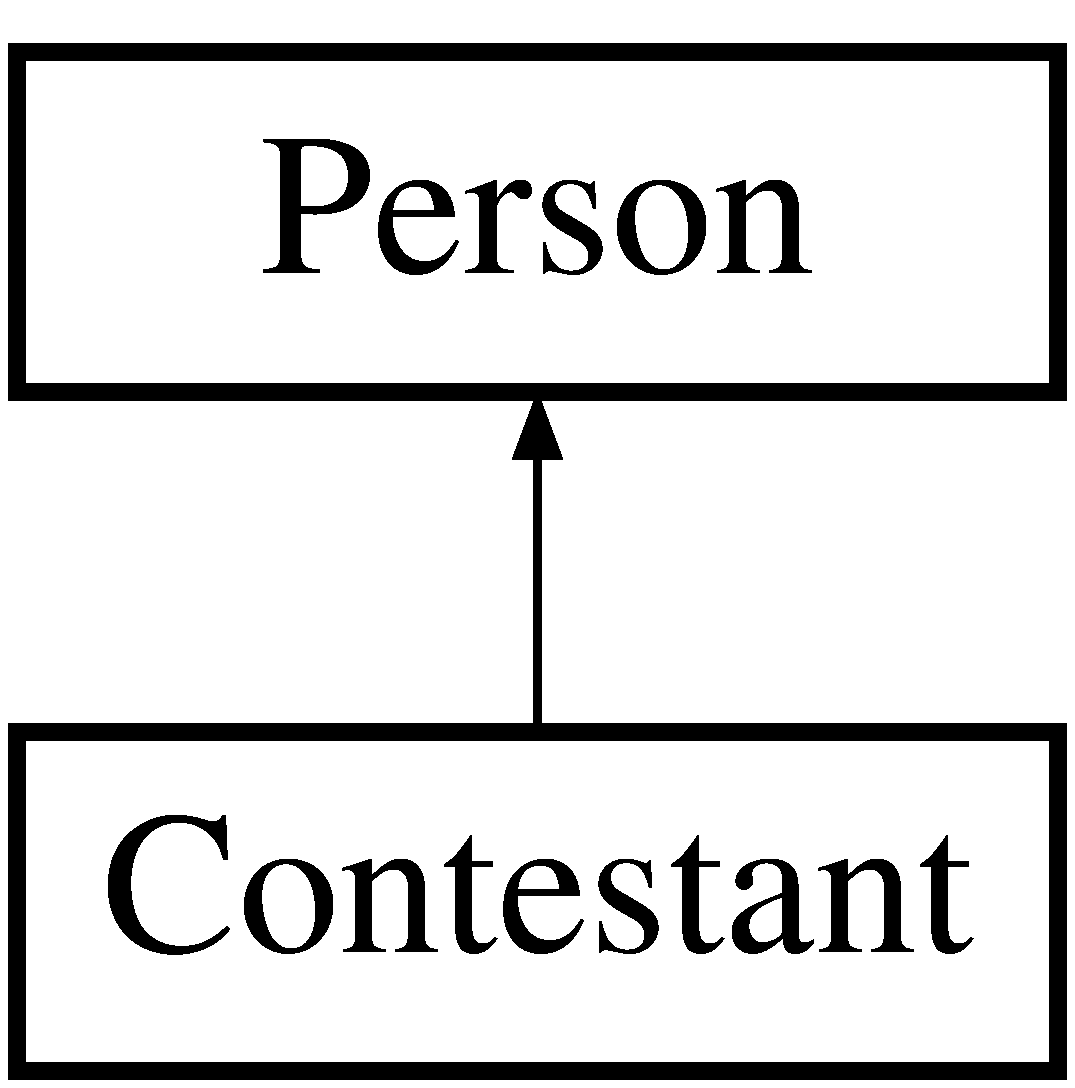
\includegraphics[height=2.000000cm]{class_contestant}
\end{center}
\end{figure}
\subsection*{Public Member Functions}
\begin{DoxyCompactItemize}
\item 
\hyperlink{class_contestant_ae7f87cb89034779cc078fd846f7dd9df}{Contestant} (string name)
\begin{DoxyCompactList}\small\item\em Construtor da classe \hyperlink{class_contestant}{Contestant}. \end{DoxyCompactList}\item 
void \hyperlink{class_contestant_a1e93516729ecfd8d49fc5dc6b8d2e01a}{setclassifications} (float a)
\begin{DoxyCompactList}\small\item\em Mete as pontuações com o valor recebido de a. \end{DoxyCompactList}\item 
float \hyperlink{class_contestant_afd136f110593d3e5dcd2bafa5454b973}{getclassifications} ()
\begin{DoxyCompactList}\small\item\em Torna acesso possível ao atributo implicitamente privado classifications. \end{DoxyCompactList}\end{DoxyCompactItemize}
\subsection*{Additional Inherited Members}


\subsection{Constructor \& Destructor Documentation}
\hypertarget{class_contestant_ae7f87cb89034779cc078fd846f7dd9df}{}\label{class_contestant_ae7f87cb89034779cc078fd846f7dd9df} 
\index{Contestant@{Contestant}!Contestant@{Contestant}}
\index{Contestant@{Contestant}!Contestant@{Contestant}}
\subsubsection{\texorpdfstring{Contestant()}{Contestant()}}
{\footnotesize\ttfamily Contestant\+::\+Contestant (\begin{DoxyParamCaption}\item[{string}]{name }\end{DoxyParamCaption})}



Construtor da classe \hyperlink{class_contestant}{Contestant}. 


\begin{DoxyParams}{Parameters}
{\em name} & Nome do concorrente (atributo vindo da classe mãe \hyperlink{class_person}{Person}) \\
\hline
\end{DoxyParams}


\subsection{Member Function Documentation}
\hypertarget{class_contestant_afd136f110593d3e5dcd2bafa5454b973}{}\label{class_contestant_afd136f110593d3e5dcd2bafa5454b973} 
\index{Contestant@{Contestant}!getclassifications@{getclassifications}}
\index{getclassifications@{getclassifications}!Contestant@{Contestant}}
\subsubsection{\texorpdfstring{getclassifications()}{getclassifications()}}
{\footnotesize\ttfamily float Contestant\+::getclassifications (\begin{DoxyParamCaption}{ }\end{DoxyParamCaption})}



Torna acesso possível ao atributo implicitamente privado classifications. 

\begin{DoxyReturn}{Returns}
Pontuações dos concorrentes 
\end{DoxyReturn}
\hypertarget{class_contestant_a1e93516729ecfd8d49fc5dc6b8d2e01a}{}\label{class_contestant_a1e93516729ecfd8d49fc5dc6b8d2e01a} 
\index{Contestant@{Contestant}!setclassifications@{setclassifications}}
\index{setclassifications@{setclassifications}!Contestant@{Contestant}}
\subsubsection{\texorpdfstring{setclassifications()}{setclassifications()}}
{\footnotesize\ttfamily void Contestant\+::setclassifications (\begin{DoxyParamCaption}\item[{float}]{a }\end{DoxyParamCaption})}



Mete as pontuações com o valor recebido de a. 


\begin{DoxyParams}{Parameters}
{\em a} & Pontuação recebida em cada fase aleatoriamente pelo público e/ou mentores \\
\hline
\end{DoxyParams}


The documentation for this class was generated from the following files\+:\begin{DoxyCompactItemize}
\item 
Person.\+h\item 
Person.\+cpp\end{DoxyCompactItemize}

\hypertarget{class_mentor}{}\section{Mentor Class Reference}
\label{class_mentor}\index{Mentor@{Mentor}}
Inheritance diagram for Mentor\+:\begin{figure}[H]
\begin{center}
\leavevmode
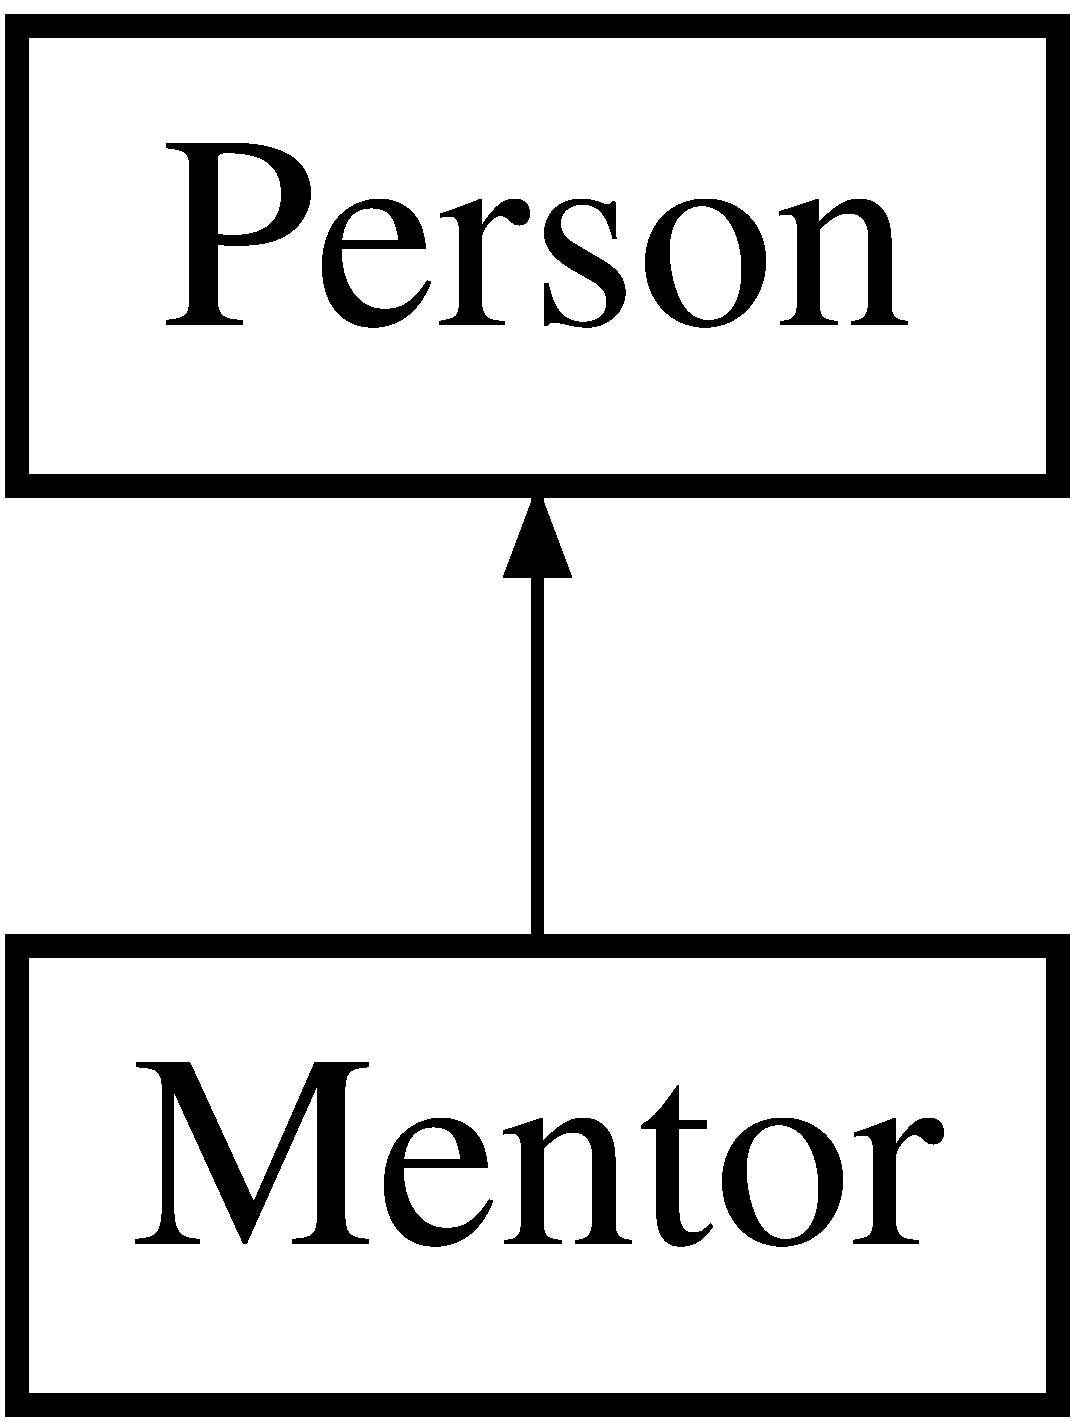
\includegraphics[height=2.000000cm]{class_mentor}
\end{center}
\end{figure}
\subsection*{Public Member Functions}
\begin{DoxyCompactItemize}
\item 
\hyperlink{class_mentor_aaeadeaf5fc979243907d643c5f6d0724}{Mentor} (string name)
\begin{DoxyCompactList}\small\item\em Construtor da classe \hyperlink{class_mentor}{Mentor}. \end{DoxyCompactList}\item 
vector$<$ \hyperlink{class_contestant}{Contestant} $\ast$ $>$ \hyperlink{class_mentor_a17141c1586d8f01dab4ad23af7281894}{get\+Team\+Blind} ()
\begin{DoxyCompactList}\small\item\em Torna acesso possível ao atributo implicitamente privado team\+Blind. \end{DoxyCompactList}\item 
vector$<$ \hyperlink{class_contestant}{Contestant} $\ast$ $>$ \hyperlink{class_mentor_a9b549210f82be5527eac9c86bf06505c}{get\+Team\+Battle} ()
\begin{DoxyCompactList}\small\item\em Torna acesso possível ao atributo implicitamente privado team\+Battle. \end{DoxyCompactList}\item 
vector$<$ \hyperlink{class_contestant}{Contestant} $\ast$ $>$ \hyperlink{class_mentor_aab229229a4b59ed74cb10a09550382e4}{get\+Team\+Final} ()
\begin{DoxyCompactList}\small\item\em Torna acesso possível ao atributo implicitamente privado team\+Final. \end{DoxyCompactList}\item 
vector$<$ \hyperlink{class_contestant}{Contestant} $\ast$ $>$ \hyperlink{class_mentor_ac05f8106cb7946dd13d3c3efafb4c3d2}{get\+Winner} ()
\begin{DoxyCompactList}\small\item\em Torna acesso possível ao atributo implicitamente privado winner. \end{DoxyCompactList}\item 
void \hyperlink{class_mentor_a56c5c3fa81d48bc50221030e3daa22b0}{add\+Team\+Blind} (\hyperlink{class_contestant}{Contestant} $\ast$c)
\begin{DoxyCompactList}\small\item\em Adiciona concorrentes ao vetor da equipa da fase Cega. \end{DoxyCompactList}\item 
void \hyperlink{class_mentor_a4b128fd072058b9c6255ef3984f79ddd}{add\+Team\+Battle} (\hyperlink{class_contestant}{Contestant} $\ast$c)
\begin{DoxyCompactList}\small\item\em Adiciona concorrentes ao vetor da equipa da fase de Batalha. \end{DoxyCompactList}\item 
void \hyperlink{class_mentor_a4e7d9c4b52211737d6135516d569ac52}{add\+Team\+Final} (\hyperlink{class_contestant}{Contestant} $\ast$c)
\begin{DoxyCompactList}\small\item\em Adiciona concorrentes ao vetor da fase Final. \end{DoxyCompactList}\item 
void \hyperlink{class_mentor_a07a8359f559b44a2fac24726f19e6dfb}{set\+Final} (\hyperlink{class_contestant}{Contestant} $\ast$c)
\begin{DoxyCompactList}\small\item\em Adiciona concorrente ao vetor do Vencedor. \end{DoxyCompactList}\end{DoxyCompactItemize}
\subsection*{Additional Inherited Members}


\subsection{Constructor \& Destructor Documentation}
\hypertarget{class_mentor_aaeadeaf5fc979243907d643c5f6d0724}{}\label{class_mentor_aaeadeaf5fc979243907d643c5f6d0724} 
\index{Mentor@{Mentor}!Mentor@{Mentor}}
\index{Mentor@{Mentor}!Mentor@{Mentor}}
\subsubsection{\texorpdfstring{Mentor()}{Mentor()}}
{\footnotesize\ttfamily Mentor\+::\+Mentor (\begin{DoxyParamCaption}\item[{string}]{name }\end{DoxyParamCaption})}



Construtor da classe \hyperlink{class_mentor}{Mentor}. 


\begin{DoxyParams}{Parameters}
{\em name} & Nome do mentor (atributo vindo da classe mãe \hyperlink{class_person}{Person}) \\
\hline
\end{DoxyParams}


\subsection{Member Function Documentation}
\hypertarget{class_mentor_a4b128fd072058b9c6255ef3984f79ddd}{}\label{class_mentor_a4b128fd072058b9c6255ef3984f79ddd} 
\index{Mentor@{Mentor}!add\+Team\+Battle@{add\+Team\+Battle}}
\index{add\+Team\+Battle@{add\+Team\+Battle}!Mentor@{Mentor}}
\subsubsection{\texorpdfstring{add\+Team\+Battle()}{addTeamBattle()}}
{\footnotesize\ttfamily void Mentor\+::add\+Team\+Battle (\begin{DoxyParamCaption}\item[{\hyperlink{class_contestant}{Contestant} $\ast$}]{c }\end{DoxyParamCaption})}



Adiciona concorrentes ao vetor da equipa da fase de Batalha. 


\begin{DoxyParams}{Parameters}
{\em c} & Apontador para um concorrente \\
\hline
\end{DoxyParams}
\hypertarget{class_mentor_a56c5c3fa81d48bc50221030e3daa22b0}{}\label{class_mentor_a56c5c3fa81d48bc50221030e3daa22b0} 
\index{Mentor@{Mentor}!add\+Team\+Blind@{add\+Team\+Blind}}
\index{add\+Team\+Blind@{add\+Team\+Blind}!Mentor@{Mentor}}
\subsubsection{\texorpdfstring{add\+Team\+Blind()}{addTeamBlind()}}
{\footnotesize\ttfamily void Mentor\+::add\+Team\+Blind (\begin{DoxyParamCaption}\item[{\hyperlink{class_contestant}{Contestant} $\ast$}]{c }\end{DoxyParamCaption})}



Adiciona concorrentes ao vetor da equipa da fase Cega. 


\begin{DoxyParams}{Parameters}
{\em c} & Apontador para um concorrente \\
\hline
\end{DoxyParams}
\hypertarget{class_mentor_a4e7d9c4b52211737d6135516d569ac52}{}\label{class_mentor_a4e7d9c4b52211737d6135516d569ac52} 
\index{Mentor@{Mentor}!add\+Team\+Final@{add\+Team\+Final}}
\index{add\+Team\+Final@{add\+Team\+Final}!Mentor@{Mentor}}
\subsubsection{\texorpdfstring{add\+Team\+Final()}{addTeamFinal()}}
{\footnotesize\ttfamily void Mentor\+::add\+Team\+Final (\begin{DoxyParamCaption}\item[{\hyperlink{class_contestant}{Contestant} $\ast$}]{c }\end{DoxyParamCaption})}



Adiciona concorrentes ao vetor da fase Final. 


\begin{DoxyParams}{Parameters}
{\em c} & Apontador para um concorrente \\
\hline
\end{DoxyParams}
\hypertarget{class_mentor_a9b549210f82be5527eac9c86bf06505c}{}\label{class_mentor_a9b549210f82be5527eac9c86bf06505c} 
\index{Mentor@{Mentor}!get\+Team\+Battle@{get\+Team\+Battle}}
\index{get\+Team\+Battle@{get\+Team\+Battle}!Mentor@{Mentor}}
\subsubsection{\texorpdfstring{get\+Team\+Battle()}{getTeamBattle()}}
{\footnotesize\ttfamily vector$<$\hyperlink{class_contestant}{Contestant}$\ast$$>$ Mentor\+::get\+Team\+Battle (\begin{DoxyParamCaption}{ }\end{DoxyParamCaption})\hspace{0.3cm}{\ttfamily [inline]}}



Torna acesso possível ao atributo implicitamente privado team\+Battle. 

\begin{DoxyReturn}{Returns}
Vetor com equipa do dado mentor na fase de Batalha 
\end{DoxyReturn}
\hypertarget{class_mentor_a17141c1586d8f01dab4ad23af7281894}{}\label{class_mentor_a17141c1586d8f01dab4ad23af7281894} 
\index{Mentor@{Mentor}!get\+Team\+Blind@{get\+Team\+Blind}}
\index{get\+Team\+Blind@{get\+Team\+Blind}!Mentor@{Mentor}}
\subsubsection{\texorpdfstring{get\+Team\+Blind()}{getTeamBlind()}}
{\footnotesize\ttfamily vector$<$\hyperlink{class_contestant}{Contestant}$\ast$$>$ Mentor\+::get\+Team\+Blind (\begin{DoxyParamCaption}{ }\end{DoxyParamCaption})\hspace{0.3cm}{\ttfamily [inline]}}



Torna acesso possível ao atributo implicitamente privado team\+Blind. 

\begin{DoxyReturn}{Returns}
Vetor com equipa do dado mentor na fase Cega 
\end{DoxyReturn}
\hypertarget{class_mentor_aab229229a4b59ed74cb10a09550382e4}{}\label{class_mentor_aab229229a4b59ed74cb10a09550382e4} 
\index{Mentor@{Mentor}!get\+Team\+Final@{get\+Team\+Final}}
\index{get\+Team\+Final@{get\+Team\+Final}!Mentor@{Mentor}}
\subsubsection{\texorpdfstring{get\+Team\+Final()}{getTeamFinal()}}
{\footnotesize\ttfamily vector$<$\hyperlink{class_contestant}{Contestant}$\ast$$>$ Mentor\+::get\+Team\+Final (\begin{DoxyParamCaption}{ }\end{DoxyParamCaption})\hspace{0.3cm}{\ttfamily [inline]}}



Torna acesso possível ao atributo implicitamente privado team\+Final. 

\begin{DoxyReturn}{Returns}
Vetor com concorrentes na fase Final 
\end{DoxyReturn}
\hypertarget{class_mentor_ac05f8106cb7946dd13d3c3efafb4c3d2}{}\label{class_mentor_ac05f8106cb7946dd13d3c3efafb4c3d2} 
\index{Mentor@{Mentor}!get\+Winner@{get\+Winner}}
\index{get\+Winner@{get\+Winner}!Mentor@{Mentor}}
\subsubsection{\texorpdfstring{get\+Winner()}{getWinner()}}
{\footnotesize\ttfamily vector$<$\hyperlink{class_contestant}{Contestant}$\ast$$>$ Mentor\+::get\+Winner (\begin{DoxyParamCaption}{ }\end{DoxyParamCaption})\hspace{0.3cm}{\ttfamily [inline]}}



Torna acesso possível ao atributo implicitamente privado winner. 

\begin{DoxyReturn}{Returns}
Vetor com vencedor da temporada 
\end{DoxyReturn}
\hypertarget{class_mentor_a07a8359f559b44a2fac24726f19e6dfb}{}\label{class_mentor_a07a8359f559b44a2fac24726f19e6dfb} 
\index{Mentor@{Mentor}!set\+Final@{set\+Final}}
\index{set\+Final@{set\+Final}!Mentor@{Mentor}}
\subsubsection{\texorpdfstring{set\+Final()}{setFinal()}}
{\footnotesize\ttfamily void Mentor\+::set\+Final (\begin{DoxyParamCaption}\item[{\hyperlink{class_contestant}{Contestant} $\ast$}]{c }\end{DoxyParamCaption})}



Adiciona concorrente ao vetor do Vencedor. 


\begin{DoxyParams}{Parameters}
{\em c} & Apontador para o concorrente que vai ganhar \\
\hline
\end{DoxyParams}


The documentation for this class was generated from the following files\+:\begin{DoxyCompactItemize}
\item 
Person.\+h\item 
Person.\+cpp\end{DoxyCompactItemize}

\hypertarget{class_person}{}\section{Person Class Reference}
\label{class_person}\index{Person@{Person}}
Inheritance diagram for Person\+:\begin{figure}[H]
\begin{center}
\leavevmode
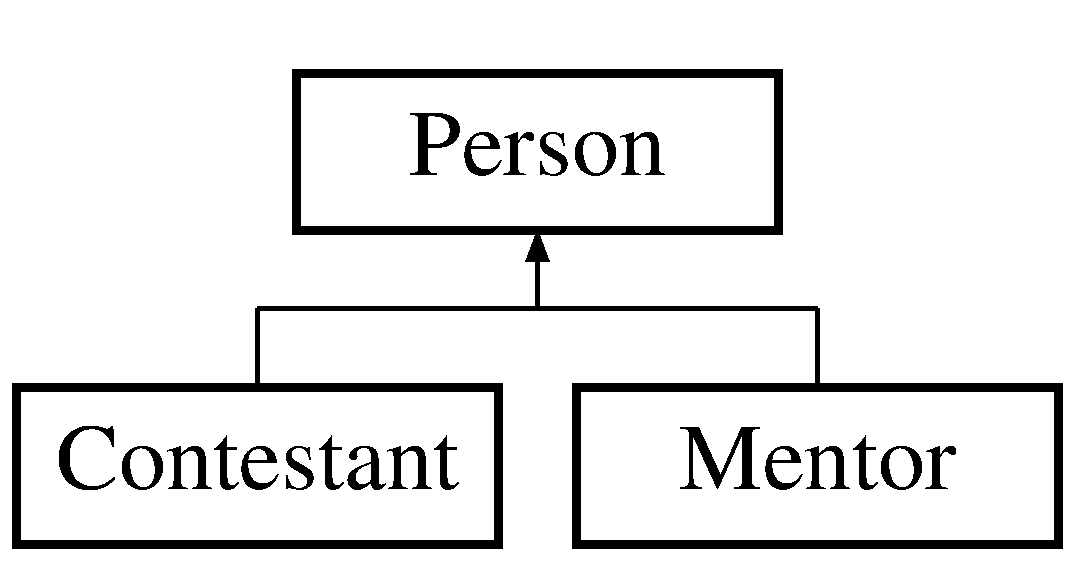
\includegraphics[height=2.000000cm]{class_person}
\end{center}
\end{figure}
\subsection*{Public Member Functions}
\begin{DoxyCompactItemize}
\item 
\hypertarget{class_person_a700ffd693321c5fe6880262acf43d4da}{}\label{class_person_a700ffd693321c5fe6880262acf43d4da} 
\hyperlink{class_person_a700ffd693321c5fe6880262acf43d4da}{$\sim$\+Person} ()
\begin{DoxyCompactList}\small\item\em Destrutor da classe \hyperlink{class_person}{Person}. \end{DoxyCompactList}\item 
\hyperlink{class_person_aba0adcb7be258cfdda603c6261a61985}{Person} (string name)
\begin{DoxyCompactList}\small\item\em Construtor da classe \hyperlink{class_person}{Person}. \end{DoxyCompactList}\item 
string \hyperlink{class_person_a1f98501a519ee5d44f53a6d6423ae67b}{get\+Name} ()
\begin{DoxyCompactList}\small\item\em Torna acesso possível ao atributo protegido name. \end{DoxyCompactList}\end{DoxyCompactItemize}
\subsection*{Protected Attributes}
\begin{DoxyCompactItemize}
\item 
\hypertarget{class_person_a669b64897b4d823a27bb5866368d4dfa}{}\label{class_person_a669b64897b4d823a27bb5866368d4dfa} 
string {\bfseries name}
\end{DoxyCompactItemize}


\subsection{Constructor \& Destructor Documentation}
\hypertarget{class_person_aba0adcb7be258cfdda603c6261a61985}{}\label{class_person_aba0adcb7be258cfdda603c6261a61985} 
\index{Person@{Person}!Person@{Person}}
\index{Person@{Person}!Person@{Person}}
\subsubsection{\texorpdfstring{Person()}{Person()}}
{\footnotesize\ttfamily Person\+::\+Person (\begin{DoxyParamCaption}\item[{string}]{name }\end{DoxyParamCaption})}



Construtor da classe \hyperlink{class_person}{Person}. 


\begin{DoxyParams}{Parameters}
{\em name} & Nome da pessoa \\
\hline
\end{DoxyParams}


\subsection{Member Function Documentation}
\hypertarget{class_person_a1f98501a519ee5d44f53a6d6423ae67b}{}\label{class_person_a1f98501a519ee5d44f53a6d6423ae67b} 
\index{Person@{Person}!get\+Name@{get\+Name}}
\index{get\+Name@{get\+Name}!Person@{Person}}
\subsubsection{\texorpdfstring{get\+Name()}{getName()}}
{\footnotesize\ttfamily string Person\+::get\+Name (\begin{DoxyParamCaption}{ }\end{DoxyParamCaption})}



Torna acesso possível ao atributo protegido name. 

\begin{DoxyReturn}{Returns}
Nome da pessoa (mentor ou concorrente) 
\end{DoxyReturn}


The documentation for this class was generated from the following files\+:\begin{DoxyCompactItemize}
\item 
Person.\+h\item 
Person.\+cpp\end{DoxyCompactItemize}

\hypertarget{class_season}{}\section{Season Class Reference}
\label{class_season}\index{Season@{Season}}
\subsection*{Public Member Functions}
\begin{DoxyCompactItemize}
\item 
\hyperlink{class_season_ae1b6176daa58d4bc4ad325f7cda57723}{Season} (vector$<$ \hyperlink{class_mentor}{Mentor} $\ast$$>$ mentors, vector$<$ \hyperlink{class_contestant}{Contestant} $\ast$$>$ contestants, vector$<$ \hyperlink{class_song}{Song} $\ast$$>$ songs)
\begin{DoxyCompactList}\small\item\em Construtor da classe \hyperlink{class_season}{Season}. \end{DoxyCompactList}\item 
\hypertarget{class_season_a8031a80200a364617e2a34e08415eaf4}{}\label{class_season_a8031a80200a364617e2a34e08415eaf4} 
void \hyperlink{class_season_a8031a80200a364617e2a34e08415eaf4}{show\+Mentors} ()
\begin{DoxyCompactList}\small\item\em Mostra na consola todos os mentores da temporada. \end{DoxyCompactList}\item 
\hypertarget{class_season_ac3d1532cd27bb5d9b74c37eee9ca11b4}{}\label{class_season_ac3d1532cd27bb5d9b74c37eee9ca11b4} 
void \hyperlink{class_season_ac3d1532cd27bb5d9b74c37eee9ca11b4}{show\+Contestants} ()
\begin{DoxyCompactList}\small\item\em Mostra na consola todos os concorrentes da temporada. \end{DoxyCompactList}\item 
\hypertarget{class_season_a16bdd5587657a529a955c817e0856394}{}\label{class_season_a16bdd5587657a529a955c817e0856394} 
void \hyperlink{class_season_a16bdd5587657a529a955c817e0856394}{addteam\+Blind} ()
\begin{DoxyCompactList}\small\item\em Associa cada música a um concorrente na primeira fase e associa cada concorrente a um mentor consoante ele vira ou não a sua cadeira. \end{DoxyCompactList}\item 
\hypertarget{class_season_a9e8562529889d23b566e65aff7ab1c4c}{}\label{class_season_a9e8562529889d23b566e65aff7ab1c4c} 
\hyperlink{class_song}{Song} $\ast$ \hyperlink{class_season_a9e8562529889d23b566e65aff7ab1c4c}{Songs\+Used} ()
\begin{DoxyCompactList}\small\item\em Determina aleatoriamente músicas a ser usadas. \end{DoxyCompactList}\item 
vector$<$ vector$<$ \hyperlink{class_contestant}{Contestant} $\ast$ $>$ $>$ \hyperlink{class_season_ac74c82ecd3f99d49a124343a4cf4d7d3}{team\+Battle\+Fase} (int a)
\begin{DoxyCompactList}\small\item\em Permite escolher os dois concorrentes que vão participar nas batalhas de um mentor. \end{DoxyCompactList}\item 
vector$<$ \hyperlink{class_song}{Song} $\ast$ $>$ \hyperlink{class_season_ad60f552ecd0508bb86cc5d41a5c10725}{team\+Battle\+Songs} ()
\begin{DoxyCompactList}\small\item\em Escolhe 7 músicas para a fase de Batalha, a partir do vetor de músicas usadas. \end{DoxyCompactList}\item 
void \hyperlink{class_season_af1202a22a58acedd837876b928b7bd0b}{Battle\+Fase} ()
\begin{DoxyCompactList}\small\item\em Mostra quem está a competir na fase de Batalha, que música está a cantar e o deixa o utilizador decidir quem ganha. \end{DoxyCompactList}\item 
\hypertarget{class_season_a8d83f3a3e9ffab62607aa01ab695dd3d}{}\label{class_season_a8d83f3a3e9ffab62607aa01ab695dd3d} 
void \hyperlink{class_season_a8d83f3a3e9ffab62607aa01ab695dd3d}{show\+Fase} ()
\begin{DoxyCompactList}\small\item\em Mostra quem chegou à fase de Galas, a música que cantam, a média da pontuação dos mentores, público e final; Mostra ainda 5 melhores concorrentes de cada gala (2 galas) \end{DoxyCompactList}\item 
\hypertarget{class_season_ad010ddb3cae5fdc5f71dd9033292ae79}{}\label{class_season_ad010ddb3cae5fdc5f71dd9033292ae79} 
void \hyperlink{class_season_ad010ddb3cae5fdc5f71dd9033292ae79}{Final\+Fase} ()
\begin{DoxyCompactList}\small\item\em Mostra quem chegou à Final, a música que cantam, a pontuação dos mentores, público e final; Mostra também vencedor (concorrente com melhor pontuação nesta fase) \end{DoxyCompactList}\end{DoxyCompactItemize}
\subsection*{Public Attributes}
\begin{DoxyCompactItemize}
\item 
\hypertarget{class_season_a4ca1bce19b8580200c0167d96cee018c}{}\label{class_season_a4ca1bce19b8580200c0167d96cee018c} 
vector$<$ \hyperlink{class_mentor}{Mentor} $\ast$ $>$ {\bfseries mentors}
\item 
\hypertarget{class_season_a2de1b335b3522e39876af68fd5213b02}{}\label{class_season_a2de1b335b3522e39876af68fd5213b02} 
vector$<$ \hyperlink{class_contestant}{Contestant} $\ast$ $>$ {\bfseries contestants}
\item 
\hypertarget{class_season_a9d6961338fb4af9426690d7d8b4cf596}{}\label{class_season_a9d6961338fb4af9426690d7d8b4cf596} 
vector$<$ \hyperlink{class_song}{Song} $\ast$ $>$ {\bfseries songs}
\item 
\hypertarget{class_season_aa3b7319b5e5ecfb4c41a40b4bedc09b1}{}\label{class_season_aa3b7319b5e5ecfb4c41a40b4bedc09b1} 
vector$<$ \hyperlink{class_song}{Song} $\ast$ $>$ {\bfseries songs\+Used}
\item 
\hypertarget{class_season_ac48fde0f957e3656a0b3463928d97dbd}{}\label{class_season_ac48fde0f957e3656a0b3463928d97dbd} 
vector$<$ \hyperlink{class_song}{Song} $\ast$ $>$ {\bfseries songsgala}
\item 
\hypertarget{class_season_ac464dcab5c001adf75c058374e77169c}{}\label{class_season_ac464dcab5c001adf75c058374e77169c} 
vector$<$ \hyperlink{class_contestant}{Contestant} $\ast$ $>$ {\bfseries gala1}
\item 
\hypertarget{class_season_a506f613439c6a7c5ad72e8cfd79e2d61}{}\label{class_season_a506f613439c6a7c5ad72e8cfd79e2d61} 
vector$<$ \hyperlink{class_contestant}{Contestant} $\ast$ $>$ {\bfseries gala2}
\item 
\hypertarget{class_season_a493540757b4629ca3575154be5caf403}{}\label{class_season_a493540757b4629ca3575154be5caf403} 
vector$<$ \hyperlink{class_contestant}{Contestant} $\ast$ $>$ {\bfseries winners}
\item 
\hypertarget{class_season_ad583038e1e0f10bca45264ba18276a04}{}\label{class_season_ad583038e1e0f10bca45264ba18276a04} 
vector$<$ \hyperlink{class_contestant}{Contestant} $\ast$ $>$ {\bfseries winners2}
\item 
\hypertarget{class_season_a4092b82e190e4689b9bb3be1d5f515cf}{}\label{class_season_a4092b82e190e4689b9bb3be1d5f515cf} 
\hyperlink{class_contestant}{Contestant} $\ast$ {\bfseries winner\+Final}
\item 
\hypertarget{class_season_a3ddf3dcac18b32a5de00cf6dd010cc1b}{}\label{class_season_a3ddf3dcac18b32a5de00cf6dd010cc1b} 
vector$<$ vector$<$ int $>$ $>$ {\bfseries n\+\_\+turned}
\end{DoxyCompactItemize}


\subsection{Constructor \& Destructor Documentation}
\hypertarget{class_season_ae1b6176daa58d4bc4ad325f7cda57723}{}\label{class_season_ae1b6176daa58d4bc4ad325f7cda57723} 
\index{Season@{Season}!Season@{Season}}
\index{Season@{Season}!Season@{Season}}
\subsubsection{\texorpdfstring{Season()}{Season()}}
{\footnotesize\ttfamily Season\+::\+Season (\begin{DoxyParamCaption}\item[{vector$<$ \hyperlink{class_mentor}{Mentor} $\ast$$>$}]{mentors,  }\item[{vector$<$ \hyperlink{class_contestant}{Contestant} $\ast$$>$}]{contestants,  }\item[{vector$<$ \hyperlink{class_song}{Song} $\ast$$>$}]{songs }\end{DoxyParamCaption})}



Construtor da classe \hyperlink{class_season}{Season}. 


\begin{DoxyParams}{Parameters}
{\em mentors} & Vetor com mentores da temporada \\
\hline
{\em contestants} & Vetor com concorrentes da temporada \\
\hline
{\em songs} & Vetor com músicas da temporada \\
\hline
\end{DoxyParams}


\subsection{Member Function Documentation}
\hypertarget{class_season_af1202a22a58acedd837876b928b7bd0b}{}\label{class_season_af1202a22a58acedd837876b928b7bd0b} 
\index{Season@{Season}!Battle\+Fase@{Battle\+Fase}}
\index{Battle\+Fase@{Battle\+Fase}!Season@{Season}}
\subsubsection{\texorpdfstring{Battle\+Fase()}{BattleFase()}}
{\footnotesize\ttfamily void Season\+::\+Battle\+Fase (\begin{DoxyParamCaption}{ }\end{DoxyParamCaption})}



Mostra quem está a competir na fase de Batalha, que música está a cantar e o deixa o utilizador decidir quem ganha. 

M\+O\+D\+I\+F\+I\+C\+A\+D\+O// \hypertarget{class_season_ac74c82ecd3f99d49a124343a4cf4d7d3}{}\label{class_season_ac74c82ecd3f99d49a124343a4cf4d7d3} 
\index{Season@{Season}!team\+Battle\+Fase@{team\+Battle\+Fase}}
\index{team\+Battle\+Fase@{team\+Battle\+Fase}!Season@{Season}}
\subsubsection{\texorpdfstring{team\+Battle\+Fase()}{teamBattleFase()}}
{\footnotesize\ttfamily vector$<$ vector$<$ \hyperlink{class_contestant}{Contestant} $\ast$ $>$ $>$ Season\+::team\+Battle\+Fase (\begin{DoxyParamCaption}\item[{int}]{a }\end{DoxyParamCaption})}



Permite escolher os dois concorrentes que vão participar nas batalhas de um mentor. 


\begin{DoxyParams}{Parameters}
{\em a} & Determina o mentor em cuja equipa estamos a fazer escolhas \\
\hline
\end{DoxyParams}
\begin{DoxyReturn}{Returns}
Vetor que contem todos os pares 
\end{DoxyReturn}
\hypertarget{class_season_ad60f552ecd0508bb86cc5d41a5c10725}{}\label{class_season_ad60f552ecd0508bb86cc5d41a5c10725} 
\index{Season@{Season}!team\+Battle\+Songs@{team\+Battle\+Songs}}
\index{team\+Battle\+Songs@{team\+Battle\+Songs}!Season@{Season}}
\subsubsection{\texorpdfstring{team\+Battle\+Songs()}{teamBattleSongs()}}
{\footnotesize\ttfamily vector$<$ \hyperlink{class_song}{Song} $\ast$ $>$ Season\+::team\+Battle\+Songs (\begin{DoxyParamCaption}{ }\end{DoxyParamCaption})}



Escolhe 7 músicas para a fase de Batalha, a partir do vetor de músicas usadas. 

\begin{DoxyReturn}{Returns}
Vetor com as 7 músicas 
\end{DoxyReturn}


The documentation for this class was generated from the following files\+:\begin{DoxyCompactItemize}
\item 
Season.\+h\item 
Season.\+cpp\end{DoxyCompactItemize}

\hypertarget{class_song}{}\section{Song Class Reference}
\label{class_song}\index{Song@{Song}}
\subsection*{Public Member Functions}
\begin{DoxyCompactItemize}
\item 
\hypertarget{class_song_a3abce584235f884768ea92d434391a8f}{}\label{class_song_a3abce584235f884768ea92d434391a8f} 
{\bfseries Song} (string name, string artist)
\item 
\hypertarget{class_song_a3f7cd6a69f4cca7ad4d8df51f7474847}{}\label{class_song_a3f7cd6a69f4cca7ad4d8df51f7474847} 
string {\bfseries get\+Name} ()
\item 
\hypertarget{class_song_a07dcbecc06e304ab0e243d612fae785d}{}\label{class_song_a07dcbecc06e304ab0e243d612fae785d} 
string {\bfseries get\+Artist} ()
\end{DoxyCompactItemize}


The documentation for this class was generated from the following file\+:\begin{DoxyCompactItemize}
\item 
Song.\+h\end{DoxyCompactItemize}

\hypertarget{class_the_voice}{}\section{The\+Voice Class Reference}
\label{class_the_voice}\index{The\+Voice@{The\+Voice}}
\subsection*{Public Member Functions}
\begin{DoxyCompactItemize}
\item 
\hypertarget{class_the_voice_a537aa6c8715a3a35bbf356155c1b237c}{}\label{class_the_voice_a537aa6c8715a3a35bbf356155c1b237c} 
void \hyperlink{class_the_voice_a537aa6c8715a3a35bbf356155c1b237c}{new\+Season} ()
\begin{DoxyCompactList}\small\item\em Gera a temporada em si. \end{DoxyCompactList}\item 
\hypertarget{class_the_voice_a2014a3032c581418fd494b2cdf21aeb3}{}\label{class_the_voice_a2014a3032c581418fd494b2cdf21aeb3} 
void {\bfseries show\+Mentors} ()
\item 
\hypertarget{class_the_voice_a1bfa4fad073a1f0bb1fef387c0da25b4}{}\label{class_the_voice_a1bfa4fad073a1f0bb1fef387c0da25b4} 
void {\bfseries Mentor\+Success} ()
\item 
\hypertarget{class_the_voice_aed5fa5d641c7d0961d56b227d2f18069}{}\label{class_the_voice_aed5fa5d641c7d0961d56b227d2f18069} 
void \hyperlink{class_the_voice_aed5fa5d641c7d0961d56b227d2f18069}{start\+Menu} ()
\begin{DoxyCompactList}\small\item\em Menu que permite ao utilizador escolher quantas temporadas quer simular e as cria. \end{DoxyCompactList}\item 
\hypertarget{class_the_voice_a165f92ac54217dcb4d95202c55820fee}{}\label{class_the_voice_a165f92ac54217dcb4d95202c55820fee} 
void {\bfseries First\+Phase\+Menu} ()
\item 
\hypertarget{class_the_voice_a88648b97a83c8fe08fb3c41faf51ffef}{}\label{class_the_voice_a88648b97a83c8fe08fb3c41faf51ffef} 
void {\bfseries Second\+Phase\+Menu} ()
\item 
\hypertarget{class_the_voice_a6a00ee6b37ae47508647ab54f4a5e6f9}{}\label{class_the_voice_a6a00ee6b37ae47508647ab54f4a5e6f9} 
void {\bfseries Third\+Phase\+Menu} ()
\item 
\hypertarget{class_the_voice_ac617cb65eb101a0648eb2611fbad2d7b}{}\label{class_the_voice_ac617cb65eb101a0648eb2611fbad2d7b} 
void {\bfseries Final\+Phase\+Menu} ()
\item 
\hypertarget{class_the_voice_a983dc00939a199ff6ce1499a96ddf5e0}{}\label{class_the_voice_a983dc00939a199ff6ce1499a96ddf5e0} 
void \hyperlink{class_the_voice_a983dc00939a199ff6ce1499a96ddf5e0}{load\+All} ()
\begin{DoxyCompactList}\small\item\em Faz com que todos os loads se efetuem. \end{DoxyCompactList}\item 
\hypertarget{class_the_voice_ab78a07d9ee3ecf2104beb1ede52038cb}{}\label{class_the_voice_ab78a07d9ee3ecf2104beb1ede52038cb} 
void \hyperlink{class_the_voice_ab78a07d9ee3ecf2104beb1ede52038cb}{load\+Songs} ()
\begin{DoxyCompactList}\small\item\em Mete num vetor todas as músicas disponíveis no documento Songs.\+txt. \end{DoxyCompactList}\item 
\hypertarget{class_the_voice_aaa446085563031cf2d125618bf39f629}{}\label{class_the_voice_aaa446085563031cf2d125618bf39f629} 
void \hyperlink{class_the_voice_aaa446085563031cf2d125618bf39f629}{load\+Contestants} ()
\begin{DoxyCompactList}\small\item\em Mete num vetor todos os concorrentes disponíveis no documento contestants.\+txt. \end{DoxyCompactList}\item 
\hypertarget{class_the_voice_adf098f29f5238611930705b4894c9957}{}\label{class_the_voice_adf098f29f5238611930705b4894c9957} 
void \hyperlink{class_the_voice_adf098f29f5238611930705b4894c9957}{load\+Mentors} ()
\begin{DoxyCompactList}\small\item\em Mete num vetor todos os mentores disponíveis no documento mentors.\+txt. \end{DoxyCompactList}\end{DoxyCompactItemize}
\subsection*{Public Attributes}
\begin{DoxyCompactItemize}
\item 
\hypertarget{class_the_voice_a1475afbddeec04e431c5f54569ea544a}{}\label{class_the_voice_a1475afbddeec04e431c5f54569ea544a} 
vector$<$ \hyperlink{class_contestant}{Contestant} $\ast$ $>$ {\bfseries contestants}
\item 
\hypertarget{class_the_voice_a781d5ce92671adb0fe6b71f445a3fbd6}{}\label{class_the_voice_a781d5ce92671adb0fe6b71f445a3fbd6} 
vector$<$ \hyperlink{class_mentor}{Mentor} $\ast$ $>$ {\bfseries mentors}
\item 
\hypertarget{class_the_voice_ac651fad37f0dc34e86d690649b24ab2d}{}\label{class_the_voice_ac651fad37f0dc34e86d690649b24ab2d} 
vector$<$ \hyperlink{class_song}{Song} $\ast$ $>$ {\bfseries songs}
\item 
\hypertarget{class_the_voice_abf86218a691f3cf1546fbb81cd575fa7}{}\label{class_the_voice_abf86218a691f3cf1546fbb81cd575fa7} 
vector$<$ \hyperlink{class_season}{Season} $>$ {\bfseries seasons}
\end{DoxyCompactItemize}


The documentation for this class was generated from the following files\+:\begin{DoxyCompactItemize}
\item 
The\+Voice.\+h\item 
Menus.\+cpp\item 
Saves.\+cpp\item 
The\+Voice.\+cpp\end{DoxyCompactItemize}

%--- End generated contents ---

% Index
\backmatter
\newpage
\phantomsection
\clearemptydoublepage
\addcontentsline{toc}{chapter}{Index}
\printindex

\end{document}
